\scanpage{60}
% block: heading
\uline{Tannakian category} (over a field $k$) \uline{with} \deleted{grou} \uline{band a diagonalizable group} $G=D(\handwritten{\unsure{\Gamma|T}})$ \handwritten{$(\Leftrightarrow\mathcal{M}$} semi-simple, and for every simple (or isotypic) object $S$ of $\handwritten{\mathcal{M}}$, of rank $d(S)$, $\operatorname{End}(S)$ is of rank $d(S)^{\handwritten{2}}\handwritten{)}$.

% block: classification and first display
Let $\deleted{M}\handwritten{\mathcal{M}}$ be this category. It is defined up to equivalence (respecting structures and constraints) by an element\inserted{\handwritten{$\xi$\begin{tikzpicture}[x=1cm,y=1cm,baseline=0cm]\draw[thin] (-.1,-.4)--(.18,.3);\end{tikzpicture}}} of $H^{\handwritten{2}}(k,G)$. On the other hand we have
\[
H^{\handwritten{2}}(k,G)\handwritten{\simeq}\operatorname{Hom}(\handwritten{\Gamma},\operatorname{Br}(k))\ ,
\]
thus $\handwritten{\mathcal{M}}$ is defined essentially by the homomorphism \deleted{cano}
\[
\handwritten{\deleted{\unsure{\xi}}u:\ \Gamma\longrightarrow}\operatorname{Br}(k)\ .
\]

% block: grading and characterization
\deleted{For every} The category $\handwritten{\mathcal{M}}$ is graded of type $\handwritten{\Gamma}$, the homogeneous objects of type $\handwritten{\Gamma}$ are\inserted{\handwritten{the objects\begin{tikzpicture}[x=1cm,y=1cm,baseline=-.1cm]\draw[thin] (0,.06).. controls (.15,-.18) and (-1.1,-.08)..(-1.25,-.3)--(-1.3,-.5);\end{tikzpicture}}} that are isotypic, thus for every $i\handwritten{\in\Gamma}$, there is exactly one simple object, up to isomorphism, $\unsure{\mathbb{E}|E}_i$, \deleted{of} homogeneous of degree $i$. (It seems that this is a second characterization of Tannakian categories with band $D(\handwritten{\Gamma})$;\inserted{\handwritten{$\Leftrightarrow$ the \unsure{direct|right|tensor|tensor} product of two isotypic objects is isotypic\begin{tikzpicture}[x=1cm,y=1cm,baseline=-.1cm]\draw[thin] (0,.06).. controls (.15,-.18) and (-1.1,-.08)..(-1.25,-.3)--(-1.3,-.5);\end{tikzpicture}}}) The degree of this element is equal to the order\inserted{$d(i)$\begin{tikzpicture}[x=1cm,y=1cm,baseline=-.1cm]\draw[thin] (0,.06).. controls (.15,-.18) and (-1.1,-.08)..(-1.25,-.3)--(-1.3,-.5);\end{tikzpicture}} of $u(i)$ in $\operatorname{Br}(k)$. Thus the ring $K(\handwritten{\mathcal{M}})$ is given by
\[
\begin{aligned}
K(\handwritten{\mathcal{M}})\handwritten{\subset}\underline{Z}\deleted{(}\handwritten{[}\handwritten{\Gamma}\handwritten{]}\ ,\\
\handwritten{\sum}n_i e^i\handwritten{\in}K(\handwritten{\mathcal{M}})\quad\handwritten{\Longleftrightarrow}\quad n_i\handwritten{\equiv}0\ (d(i))\quad\text{for every }i\handwritten{\in\Gamma}
\end{aligned}
\]
The canonical basis of $K(\handwritten{\mathcal{M}})$ formed by the simple objects being formed of the $d(i)e^i$. If $M_i$ is the simple object of \deleted{weight} degree $i$, then $\operatorname{End}(M_i)$ is the skew field \deleted{of over} with center $k$ whose invariant in $\operatorname{Br}(k)$ is $u(i)$.

% block: cancelled paragraph
\deleted{In terms of a system of generators $({}_i)_{i\,\unsure{I|\in I}}$ of $I$, \deleted{and}(of a system of \deleted{simple}\inserted{isotypic} objects \deleted{$\unsure{M|\mathbb{M}}_i$} \deleted{of type} degree $i$)and of the}

\figure{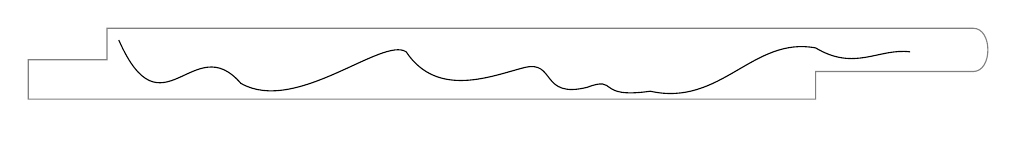
\begin{tikzpicture}[x=1cm,y=1cm]\draw[thin,gray] (0,0)--(0,.4)--(1,.4)--(1,.8)--(12,.8).. controls (12.25,.8) and (12.25,.25)..(12,.25)--(10,.25)--(10,-.1)--(0,-.1)--cycle;\draw (1.15,.65).. controls (1.7,-.6) and (2.1,.8)..(2.7,.1).. controls (3.4,-.3) and (4.5,.7)..(4.8,.5).. controls (5.2,-.1) and (5.9,.2)..(6.3,.3).. controls (6.7,.4) and (6.5,-.1)..(7.1,.05).. controls (7.5,.2) and (7.2,-.1)..(7.9,0).. controls (8.8,-.2) and (9.2,.7)..(10,.55).. controls (10.5,.25) and (10.8,.55)..(11.2,.5);\end{tikzpicture}}

% block: free group case
If $\Gamma=Z^{(I)}$,\inserted{i.e. $G=G_m^I$,\begin{tikzpicture}[x=1cm,y=1cm,baseline=-.1cm]\draw[thin] (0,.06).. controls (.15,-.18) and (-1.1,-.08)..(-1.25,-.3)--(-1.3,-.5);\end{tikzpicture}} the datum of $u$\inserted{i.e. of $\handwritten{\xi}$\begin{tikzpicture}[x=1cm,y=1cm,baseline=-.1cm]\draw[thin] (0,.06).. controls (.15,-.18) and (-1.1,-.08)..(-1.25,-.3)--(-1.3,-.5);\end{tikzpicture}} amounts to the datum of elements $\handwritten{\xi}_i\handwritten{\in}\operatorname{Br}(k)$. Choosing for every $i$ a nonzero isotypic object of degree $i$, say $E_i$, and denoting by $A_i=\operatorname{End}(\deleted{\unsure{A|M}}\handwritten{M}_i)$ the associated Azymaya algebra,\inserted{of class $\handwritten{\xi}_i$,\begin{tikzpicture}[x=1cm,y=1cm,baseline=-.1cm]\draw[thin] (0,.06).. controls (.15,-.18) and (-1.1,-.08)..(-1.25,-.3)--(-1.3,-.5);\end{tikzpicture}} one reconstructs (up to unique equivalence\deleted{)} respecting everything)
% archive sheet number: 59
